\chapter{Basic Neural Network Architectures in Keras}

\section{Common Code for Neural Nets}


\subsection{Train models with Saved intermediates}


Following is the basic code to run when training the neural Network.

\begin{lstlisting}[style=py]
model.fit(x=X_train, y=X_train, epochs=25,
validation_data=[X_validation, Y_validation],
callbacks=[keras_utils.ModelSaveCallback(model_filename),
        keras_utils.TqdmProgressCallback()],
verbose=0,
initial_epoch=last_finished_epoch or 0)
\end{lstlisting}

And this is the code to load a presaved checkpoint of the model and start traininf from the last completed epoch. The keras\_utils file is available in the snippets, and makes these callbacks available.

\begin{lstlisting}[style=py]
def load_checkpoint(last_epoch)
    model_filename = 'model.{0:03d}.hdf5'
    last_finished_epoch = None
    if last_epoch is not None:
        s = keras_utils.reset_tf_session()
        last_finished_epoch = 4
        model = keras.models.load_model(model_filename.format(last_finished_epoch))
\end{lstlisting}

Following this, we always save our weights in a file, and then load from it, as follows:
\begin{lstlisting}[style=py]
encoder.save_weights("encoder.h5")
decoder.save_weights("decoder.h5")
\end{lstlisting}



\section{AutoEncoders}

\subsection{Convolutional Autoencoders}

Here is the code for the setting up a Convolutional AutoEncoders. Follows a 4 layer Conv-Pool and then 1 Dense layer architecture to encode, then a dense layer followed by Transpose Convolutional layers to decode.

\lstinputlisting[style=py]{snippets/ml_architectures/convolutional_autoencoder.py}



\section{Recurrent Units}


\subsection{Long Short Term Memory (LSTM)}

\begin{figure}[H]
	\centering
	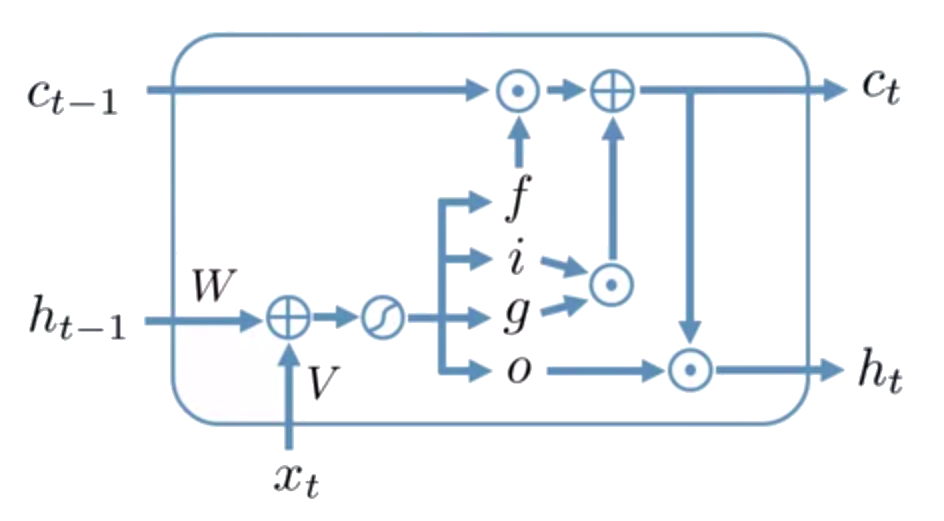
\includegraphics[width=0.9\linewidth]{img/aml/lstm-schematic.png}
	\caption{Schematic Diagram of LSTM}
	\label{fig:lstm-schmatic}
\end{figure}

\subsubsection{Update Equations}

Following are the update equations for an LSTM. There are 3 gates, the Input Gate (which saves to cell memory), and Output Gate (which loads from cell memory) and a Forget Gate (which clears up cell memory). In addition a Gate Value is generated, which is what gets stored in the memory during input. All these get computed from the catenation of the previous hidden state and the current input.

\begin{eqnarray}
	g_t &=& \tilde{f}(W_g \cdot \text{Concat}[x_t, h_{t - 1}] + b_g) \\
	f_t &=& \sigma(W_f \cdot \text{Concat}[x_t, h_{t - 1}] + b_f) \\
	i_t &=& \sigma(W_i \cdot \text{Concat}[x_t, h_{t - 1}] + b_i) \\
	o_t &=& \sigma(W_o \cdot \text{Concat}[x_t, h_{t - 1}] + b_o) \\
	c_t &=& f_t \cdot c_{t - 1} + i_t \cdot g_t \\
\end{eqnarray}

The hidden state is the output, which can be available as the entire sequence or only at the end. A dense layer or any other can be used on top of it to compute some other output $y_t$.

\subsubsection{Management of Gradients}

Since the memory cell connections are like a skip connection if there is no update/forget operation, the gradients do not vanish as easily.


\subsection{Gated Recurrence Unit (GRU)}

\begin{figure}[H]
	\centering
	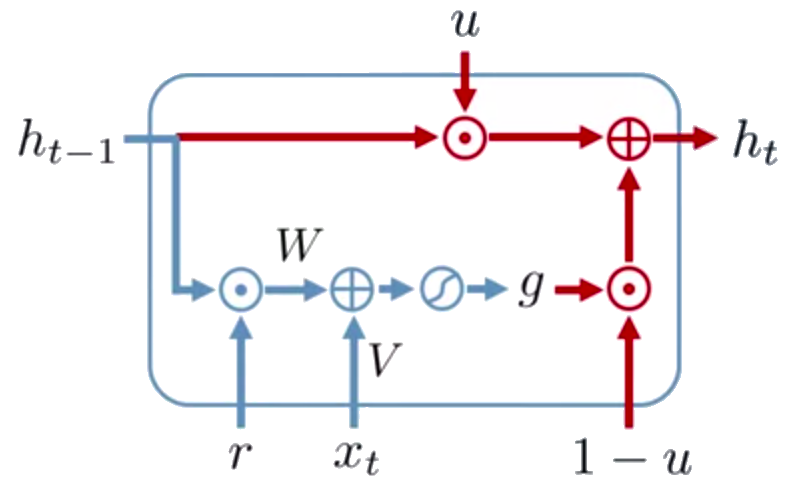
\includegraphics[width=0.9\linewidth]{img/aml/gru-schematic.png}
	\caption{Schematic Diagram of GRU}
	\label{fig:gru-schmatic}
\end{figure}
